% DesiDiet Neo4j knowledge-graph schema (publication figure source)
\documentclass[tikz,border=5pt]{standalone}
\usepackage[T1]{fontenc}
\usepackage{lmodern}
\usetikzlibrary{arrows.meta,positioning,calc}
\definecolor{navy}{HTML}{17365D}
\definecolor{blue}{HTML}{2F6690}
\definecolor{teal}{HTML}{197278}
\definecolor{gold}{HTML}{C18C24}
\definecolor{graytext}{HTML}{48515B}
\begin{document}
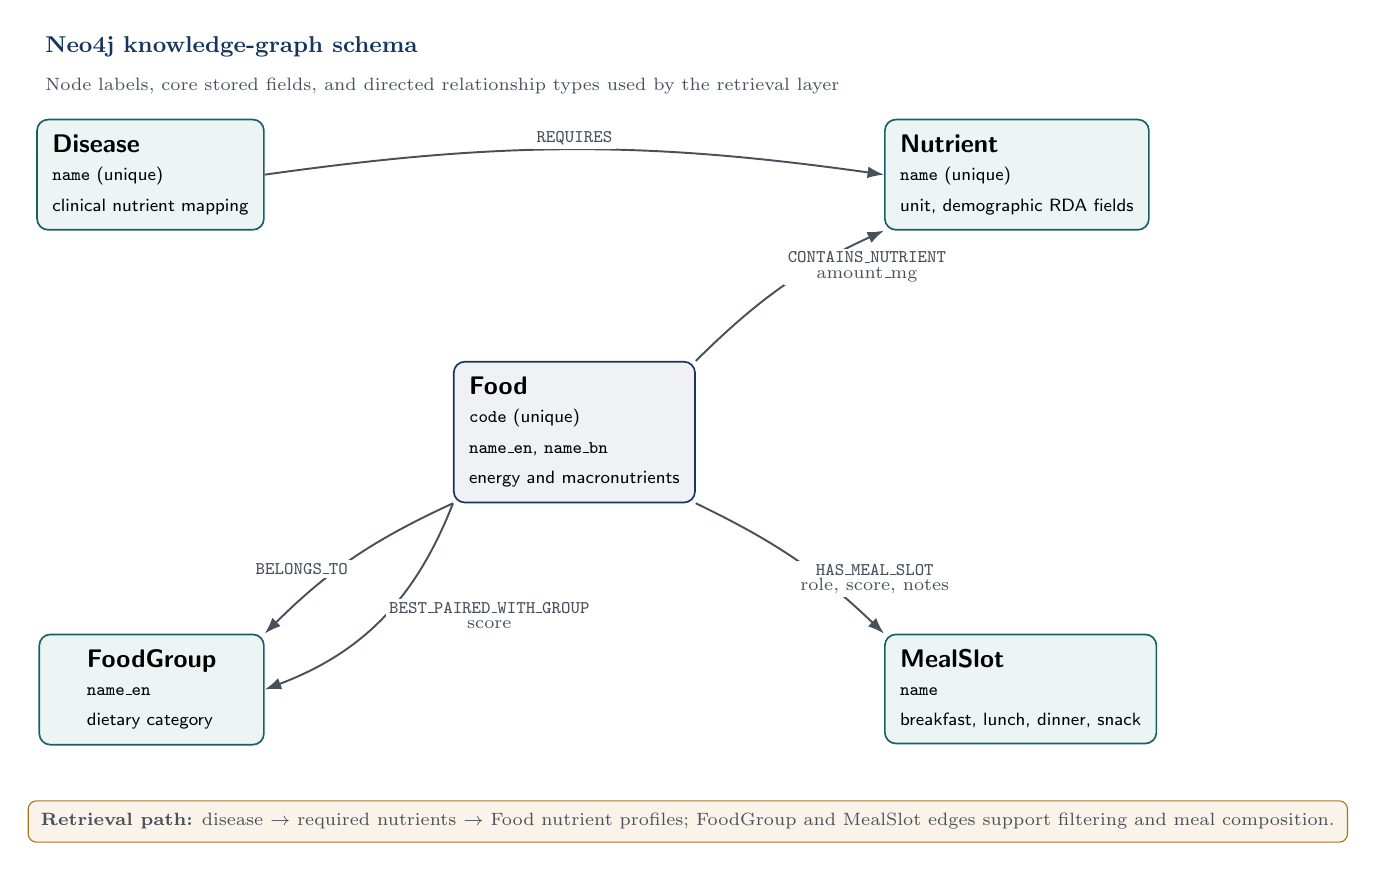
\begin{tikzpicture}[
  font=\sffamily,
  scale=.92, transform shape,
  entity/.style={draw=navy, fill=navy!7, rounded corners=4pt, minimum width=3.1cm, minimum height=1.45cm, align=left, inner sep=6pt, line width=.6pt},
  entity2/.style={draw=teal!85!black, fill=teal!8, rounded corners=4pt, minimum width=3.1cm, minimum height=1.25cm, align=left, inner sep=6pt, line width=.6pt},
  edge/.style={-{Latex[length=2.1mm,width=1.5mm]}, line width=.7pt, draw=graytext},
  rel/.style={font=\scriptsize\ttfamily, fill=white, inner sep=1.4pt, text=graytext, align=center},
  title/.style={font=\small\bfseries, text=navy},
  props/.style={font=\scriptsize, text=graytext}
]
\node[entity] (food) {\textbf{Food}\\[-1pt]\scriptsize\texttt{code} (unique)\\\scriptsize\texttt{name\_en}, \texttt{name\_bn}\\\scriptsize energy and macronutrients};
\node[entity2, above right=18mm and 26mm of food] (nutrient) {\textbf{Nutrient}\\[-1pt]\scriptsize\texttt{name} (unique)\\\scriptsize unit, demographic RDA fields};
\node[entity2, above left=18mm and 26mm of food] (disease) {\textbf{Disease}\\[-1pt]\scriptsize\texttt{name} (unique)\\\scriptsize clinical nutrient mapping};
\node[entity2, below left=18mm and 26mm of food] (group) {\textbf{FoodGroup}\\[-1pt]\scriptsize\texttt{name\_en}\\\scriptsize dietary category};
\node[entity2, below right=18mm and 26mm of food] (slot) {\textbf{MealSlot}\\[-1pt]\scriptsize\texttt{name}\\\scriptsize breakfast, lunch, dinner, snack};

% Relationship topology
\draw[edge] (food.north east) to[bend left=10] node[rel, above right] {CONTAINS\_NUTRIENT\\[-2pt]\normalfont\scriptsize amount\_mg} (nutrient.south west);
\draw[edge] (disease.east) to[bend left=8] node[rel, above] {REQUIRES} (nutrient.west);
\draw[edge] (food.south west) to[bend right=10] node[rel, below left] {BELONGS\_TO} (group.north east);
\draw[edge] (food.south west) to[bend left=24] node[rel, pos=.48, right] {BEST\_PAIRED\_WITH\_GROUP\\[-2pt]\normalfont\scriptsize score} (group.east);
\draw[edge] (food.south east) to[bend left=9] node[rel, below right] {HAS\_MEAL\_SLOT\\[-2pt]\normalfont\scriptsize role, score, notes} (slot.north west);

% Top annotations
\node[title, anchor=west] at ($(disease.north west)+(0,1.0)$) {Neo4j knowledge-graph schema};
\node[props, anchor=west] at ($(disease.north west)+(0,.45)$) {Node labels, core stored fields, and directed relationship types used by the retrieval layer};
\node[draw=gold!85!black, fill=gold!10, rounded corners=3pt, align=left, inner sep=5pt, font=\scriptsize, text=graytext, anchor=west] at ($(group.south west)+(-.15,-1.05)$) {\textbf{Retrieval path:} disease $\rightarrow$ required nutrients $\rightarrow$ Food nutrient profiles; FoodGroup and MealSlot edges support filtering and meal composition.};
\end{tikzpicture}
\end{document}
